\documentclass[11pt]{article}
\usepackage{graphicx}
\usepackage[margin=1in]{geometry}

\title{ECE 545 Assignment 2 -- Breaking AES through DPA}
\author{Henry Su}
\date{}

\begin{document}
\maketitle

\section*{Task 1 -- Analyzing the power trace}

\subsection*{Figure 1}
\begin{center}
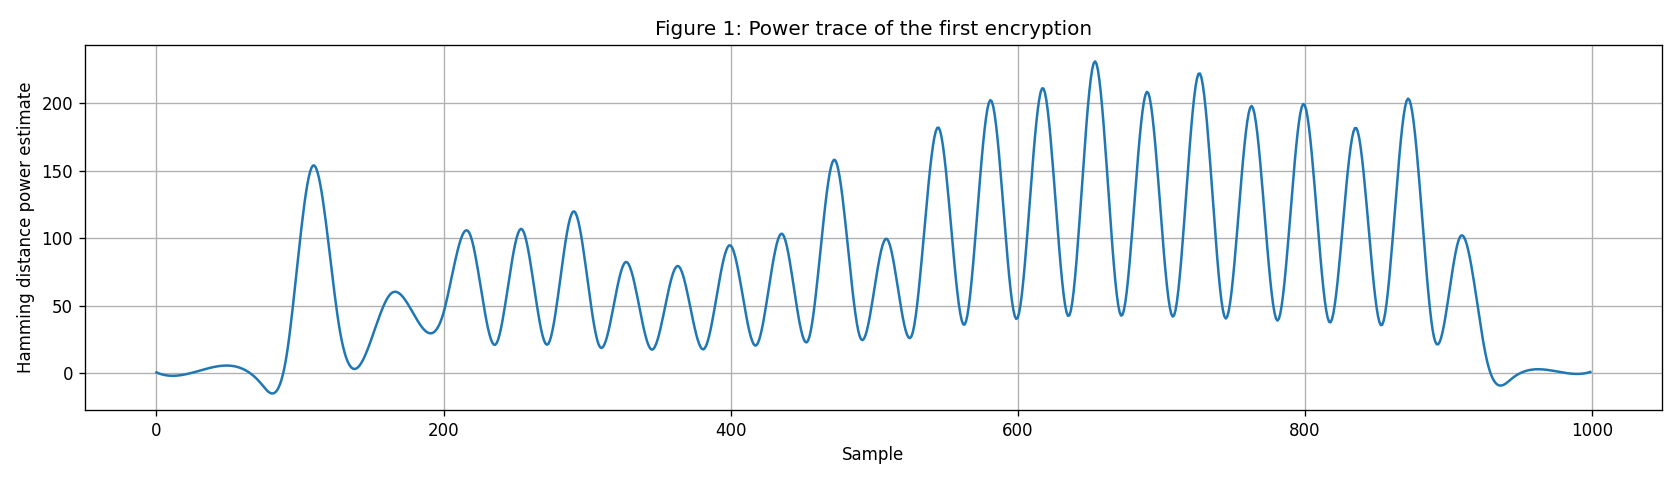
\includegraphics[width=\textwidth]{figure1_first_trace.png}
\end{center}

\subsection*{Question 1}
Analyze the power trace you plotted in Task 1 (Figure 1). What are the peaks in the trace? How is AES implemented?

\bigskip
\noindent 22 peaks.
Peaks 1 through 11 seem to be before any encryption starts. FSM starts 11 clock cycles computing the entire key schedule which is independent of the plaintext.
Peaks 12 through 22 now seems to have state\_reg\_0 .. 3 update every cycle too simultaneously while computing the key schedule. 12 through 22 seem to be actual encryption with mixcolumns mixing bits around.
Last peak is probably round 10 that skips mixcolumns.

\subsection*{Subtask C -- pre-processing}
Before we proceed to DPA, think of a good pre-processing step to make the attack more successful.

\bigskip
\noindent If traces are misaligned then correlating across traces would smear the real signal. A good pre processing step would be trace alignment and making sure or checking if every trace lines up sample for sample.

\section*{Task 2 -- Performing the DPA attack}

\subsection*{Subtask A -- target operation}
Let's execute the DPA attack using Pearson's correlation test. First, think of an easy target operation for the DPA and, second, consider the number of bits to be estimated by DPA at a time.

\bigskip
\noindent Let's target the last round using the known ciphertext. Round 10 doesn't seem to use mixcolumns so the output byte depends on exactly one s-box output and one round 10 key byte per byte which makes it a lot more simple.

\subsection*{Question 2}
What is a good power model for the target operation? Justify it.

\bigskip
\noindent My answer for this would be hamming distance. It counts how many bit flips between a register's old value and new value. For round 10, old value is the unknown pre final round byte and new value is the known ciphertext byte. We can guess the key and use it to compute a candidate for the old value and count the hamming distance. I tried the simpler model but the real key was hard to decipher from the noise.

\subsection*{Figure 2}
\begin{center}
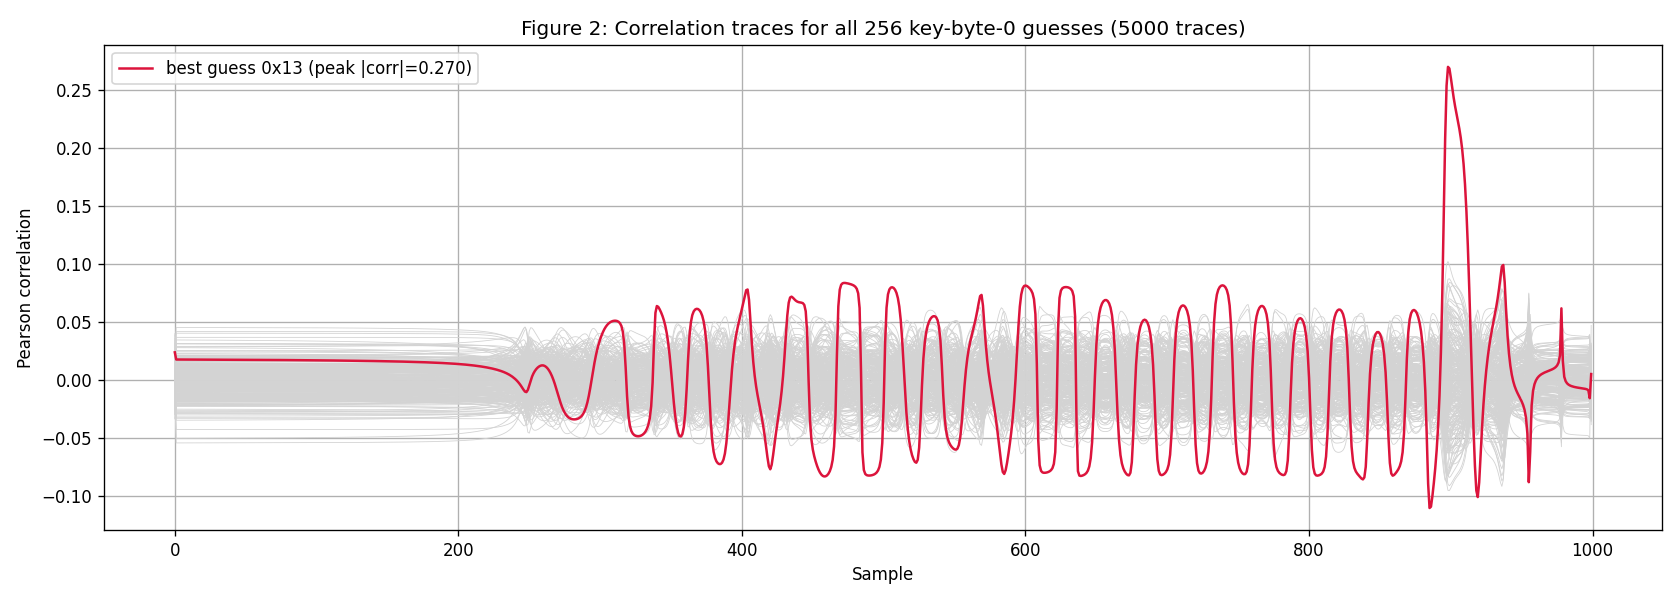
\includegraphics[width=\textwidth]{figure2_all_guesses_byte0.png}
\end{center}

\subsection*{Figure 3}
\begin{center}
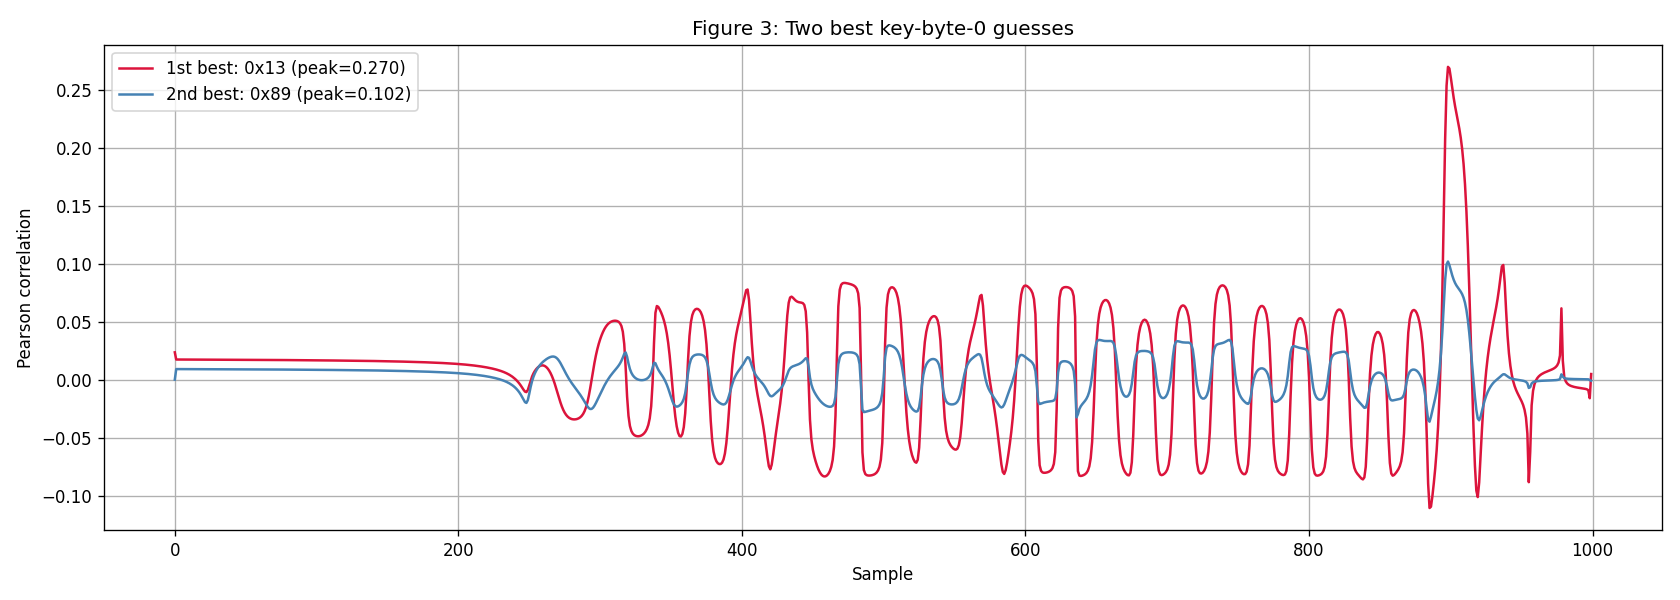
\includegraphics[width=\textwidth]{figure3_two_best_byte0.png}
\end{center}

\subsection*{Question 3}
Considering the two cases from above (Figure 3), which one is more likely to be the correct key guess? Why do you specifically see these two results?

\bigskip
\noindent I'm thinking whichever guess has the largest magnitude and stands clearly above the noise is the strongest guess. I'm seeing these two results because a wrong guess can correlate strongly in the opposite direction just by how the bits interact. With that I have to check both the positive and negative candidates in magnitude and pick whichever one is the biggest.

\subsection*{Question 4}
What is the maximum leak point? Since you are working with an interpolated power trace without timestamp data, a sample number would work.

\bigskip
\noindent [TODO: fill in -- sample 898 out of 1000, from the Figure 2/4 analysis]

\subsection*{Figure 4}
\begin{center}
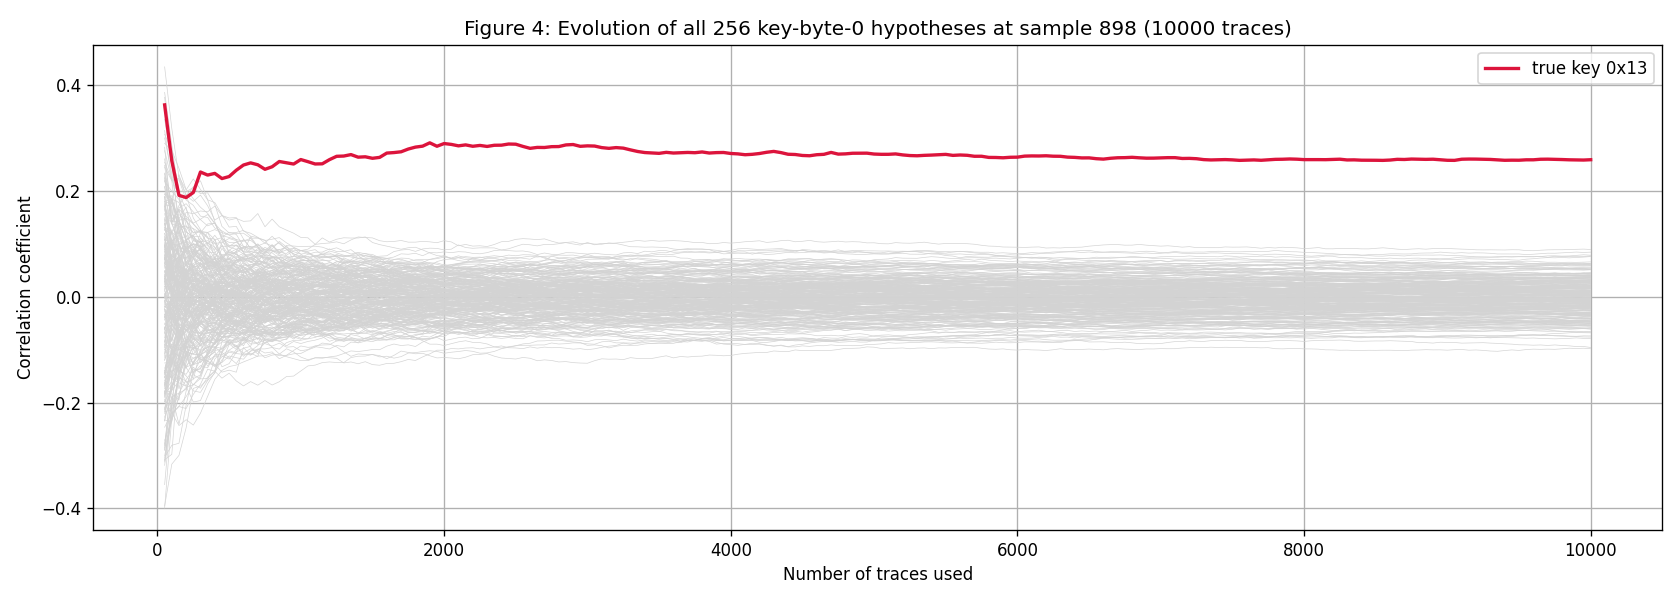
\includegraphics[width=\textwidth]{figure4_evolution_10k.png}
\end{center}

\subsection*{Question 5}
Starting at how many traces, does the key guess with maximum correlation show highest correlation?

\bigskip
\noindent N = 300 traces.

\subsection*{Question 6}
Apply the DPA on the entire key. What is the 128-bit AES secret key?

\bigskip
\noindent The recovered 128 bit AES secret key is

\begin{center}
00 01 02 03 04 05 06 07 08 09 0a 0b 0c 0d 0e 0f
\end{center}

\section*{Task 3 -- Evaluating the DPA attack}

\subsection*{Question 7}
What is the mean time to disclosure, i.e. average number of traces required to extract the key for your DPA attack?

\bigskip
\noindent For each of the 16 key bytes we find the smallest N at which that byte's correct guess first becomes the top guess, then average across all 16 bytes. Mean time to disclosure $\approx$ 722 traces.

\subsection*{Question 8}
Compare this with the theoretical cryptanalysis (i.e. brute-force attack) of AES, what is the reduction ratio in the number of traces required to break AES? Why is DPA so powerful?

\bigskip
\noindent Brute force would need about $2^{127}$ attempts to find the 128 bit key, about $1.7\times10^{38}$ guesses. This DPA attack only needed $10^2$--$10^3$ power traces to recover the entire key, which is a lot better -- about $10^{35.7}$ reduction ratio.

DPA is powerful because it doesn't treat the 128 bit key as one giant unknown thing but targets an 8 bit operation at a time so we can slowly isolate every byte during every round.

\section*{Bonus Questions}

\subsection*{Question 9}
Did you use AI in any form to complete the assignment?

I used a little bit of AI to help me write the print statements and set up the function declarations, as well as the SBOX array. Most logic I tried writing myself and when I ran into a wall Id ask AI for pointers. So I did use AI.

\bigskip

\subsection*{Question 10 (Optional)}
How long did it take for you to complete questions 1 to 8?

1.5 Hour - 2 hour ish.

\bigskip

\end{document}
